\begin{apendicesenv}
	% Imprime uma página indicando o início dos apêndices
	\partapendices
	\begin{landscape}
		\chapter{Material de apoio}
		\begin{figure}[h]
			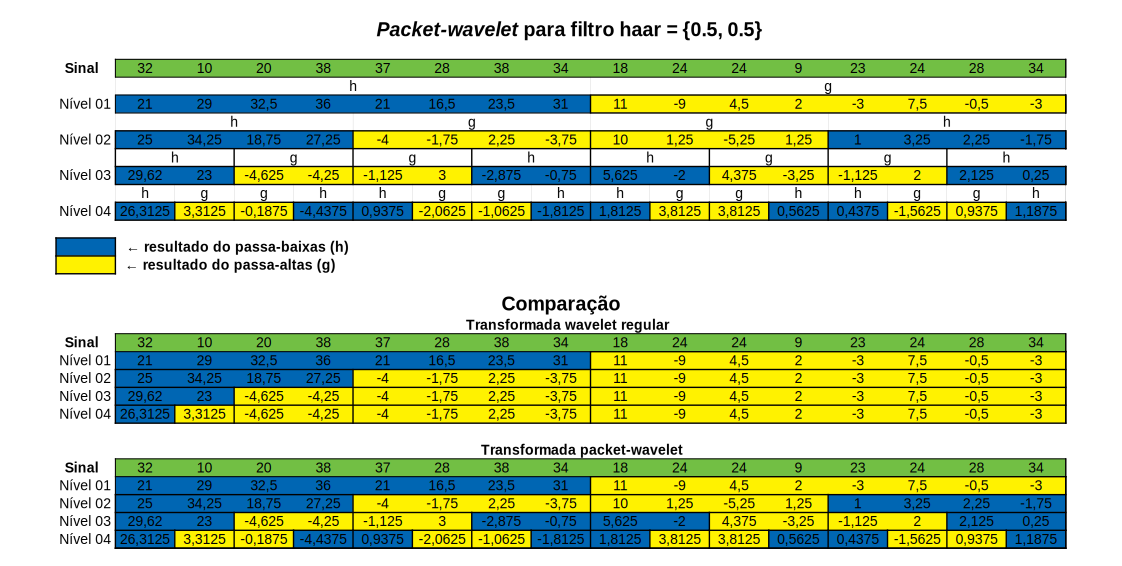
\includegraphics[width=.9\linewidth]{images/haarWaveletExamples.pdf}
			\caption{Demostração numérica das transformadas Wavelet e Wavelet packet: Por razões didáticas a \textit{Wavelet} Haar foi considerada como tendo os valores $1/2$ e $-1/2$}
			\label{fig:haarWaveletExamples}
		\end{figure}
	\end{landscape}
	\chapter{Recursos na web}
		\par Para realização deste trabalho foram produzidos variados textos (este incluso) e códigos, é recomendada a consulta dos códigos fontes utilizados nos procedimentos como complemento que, se espera, melhore o entendimento dos assuntos discutidos.
		
		\par Uma atenção especial deve ser dada ao diretório localizado em \textit{\textbf{/src/lib}} que contém todas as bibliotecas criadas e referenciadas para resolver os problemas surgidos e também ao \textit{\textbf{/src/experiments}} que contém os procedimentos já descritos.
				
		\par Em \textit{\textbf{/soundSamples}} se encontra a base de dados com os áudios originais e tratados.
		
		\par Alguns \textit{scripts} foram desenvolvidos para facilitar o tratamento dos arquivos de áudio, os mesmos se encontram em \textbf{\textit{/src/scripts}}.
		
		\par Por fim a parte escrita pode ser consultada em \textit{\textbf{/documentation}}.
		
		\par Todos esses materiais estão sob licença de código aberto (GPLv3) e são livres para uso não comercial acesse   \href{https://github.com/ensismoebius/voiceSpoofingDetectionWavelet}{https://github.com/ensismoebius/voiceSpoofingDetectionWavelet} para mais informações.
\end{apendicesenv}